%\newpage
\section{Datamining} \label{sec:datamining}

For our project we have decided to test ten different classification algorithms. K nearest Neighbors, Random Forest, Decision Tree, Support vector machine, logistic regression, XGBoost, and four naïve bayes classifiers based on Bernoulli complement gaussian multinomial.

These ten classification algorithms will be evaluated to determine which one fulfills our two criterions best. The first criterion is that the model should be as simple as possible like stated by the Occam’s razor law. The reason for this is that we want our model to be used universally by doctors but also by patients who may not have great expertise in medical practice. The second criterion is precision, in order to avoid possible Type 2 errors (a patient with a heart disease is diagnosed as negative) in the diagnosis.

Besides the before mentioned use of scalers, imputers and samplers we additionally apply a variety of classifier specific hyperparameters. We combine both in a grid search approach while training and testing the models. For the KNN we added two hyperparameters for calculating new instances based on their nearest neighbor. The options were simply taking the majority class or weighting the values by distance. Since KNN relies on some kind of a distance measure we included the options for using the Manhattan distance and the Euclidian distance. Moreover, we tested nearest neighbor values from 2 to 97 (moving in 5-unit steps). Random Forest was tested with numbers of estimators ranging from 10 to 90 (10-unit steps), a maximum depth of null, 2, 6 and 10 and a minimum number of instances per leaf of 2, 6, and 10. Decisions Trees were tested with both the gini index and entropy as impurity measures while the values for maximum tree depth and minimum instances per leaf were the same as for Random Forest. In the case of logistic regression, we added the same distance options as for KNN. For SVC we tested for C values ranging from 120 to 160 (20-unit steps), as well as the gamma values 0.0001, 0.001, 0.01 and the kernel options linear, polynomial, sigmoidal and radial basis function. For the four naïve bayes estimators we applied alpha values from 0 to 19.5 (0.5-unit steps). 

For all models we choose a majority class baseline approach. In our case this means that having a heart disease will be the models` baseline. Due to the small number of observations in our dataset, we chose to train and test our models by using a nested stratified cross validation with 10-folds, to use as much data as possible for both the training and testing of our models. 

Applying all these methods result in a large number of trained models (approx. 45.360.000). In order to be able to still discuss different models we have decided to evaluate the one model for each classification algorithm that comes closest to our criterions. Therefore, for each classification algorithm we chose the one model that accomplished the highest average level of accuracy, while minimizing the average deviation (size of accuracy confidence intervals) and the number of Type 2 errors. According to Occams Razor we favoured models with a low number of columns. Therefore models with a low number in percentageToBeDropped were chosen.

\Cref{table:modelresults} includes these best models and displays those models with their used algorithms, scaler, imputer, sampler, in addition to some prediction metrics.  


% INSERT TABLE

\begin{table}[]
\begin{adjustwidth}{-3cm}{}

\begin{footnotesize}
\begin{tabular}{|l|l|l|l|l|l|l|l|l|l|l|l|}
\hline
\textbf{Classifier} & \textbf{Scaler}   & \textbf{Sampler}   & \textbf{Type 2} & \textbf{Acc.} & \textbf{Conf. interval} & \textbf{Pre.} & \textbf{Rec.} & \textbf{F1} & \textbf{Conf. interval} & \textbf{MPD} \\ \hline
KNN                                & none                 & none               & 70              & 76.29         & {[}76.25, 76.32{]}   & 0.78           & 0.77        & 0.77         & {[}0.73, 0.80{]}      & 0                                                    \\ \hline
XGB                                & Normalizer           & RUS 				   & 109             & 76.54         & {[}76.49, 76.59{]}    & 0.78           & 0.77        & 0.76         & {[}0.70, 0.82{]}      & 75                                                   \\ \hline
Random Forest                      & StandardScaler       & none               & 79              & 78.33         & {[}78.27, 78.39{]}   & 0.82           & 0.79        & 0.78         & {[}0.70, 0.85{]}     & 100                                                  \\ \hline
Decision Tree                      & none                 & none               & 73              & 76.70         & {[}76.67, 76.74{]}    & 0.79           & 0.78        & 0.77         & {[}0.73, 0.81{]}     & 0                                                    \\ \hline
SVC                                & PowerTransformer     & none               & 92              & 77.87         & {[}77.82, 77.92{]}   & 0.80           & 0.78        & 0.77         & {[}0.71, 0.83{]}     & 20                                                   \\ \hline
NB (bernoulli)            & StandardScaler       & none               & 111             & 79.07         & {[}79.02, 79.11{]}   & 0.80           & 0.79        & 0.79         & {[}0.74, 0.83{]}      & 8                                                    \\ \hline
NB (complement)           & MinMaxScaler         & none               & 78              & 77.48         & {[}77.44, 77.53{]}   & 0.78            & 0.78         & 0.78         & {[}0.74, 0.82{]}     & 100                                                  \\ \hline
NB (gaussian)             & Normalizer           & none               & 233             & 70.46         & {[}70.42, 70.49{]}   & 0.76           & 0.69        & 0.67         & {[}0.63, 0.71{]}     & 20                                                   \\ \hline
NB (multinomial)          & MinMaxScaler         & none               & 99              & 76.46         & {[}76.43, 76.50{]}   & 0.77           & 0.77        & 0.77         & {[}0.73, 0.80{]}     & 100                                                  \\ \hline
logistic regression                & Normalizer           & none               & 75              & 76.03         & {[}75.99, 76.06{]}   & 0.78           & 0.77         & 0.76         & {[}0.73, 0.80{]}     & 0                                                    \\ \hline
\end{tabular}

\begin{adjustwidth}{+3cm}{}
\begin{center}
\centering
RUS = random under sampler, MPD = minimum percentage to be dropped
\end{center}
\end{adjustwidth}
\end{footnotesize}
\caption{Best models for every classification algorithm} 
\label{table:modelresults}
	
\end{adjustwidth}
\end{table}

While all models have accuracies between 70\% and 79\%, with small confidence intervals respectively, they show great discrepancies in both the total Type 2 errors and the minimum percentage to be dropped. The model with the lowest Type 2 error is the one with KNN (Type 2 = 70), the one with the highest uses naïve bayes gaussian (Type 2 = 233), which is also the model that shows the lowest average accuracy. A total of three models have a minimum percentage to be dropped of 0\% (only features that do not have missing values are maintained), KNN, decision tree and logistic regression. The models with the highest minimum percentage to be dropped which is 100\% are the ones using the Random Forest, and the naïve bayes models using multinomial and complement. 

Based on the different model results and our predefined criterion we argue that the best model for classifying whether somebody has a heart disease or not is the model which uses the decision tree, followed closely by the before discussed KNN model.

The decision tree uses no scaler nor sampler and uses the simple imputer and as an additional hyperparameters the gini index was used as impurity measure, while the maximum tree depth was set to none, with a minimum instances per leaf value of 2. The total depth of the tree is 5. Overall, the decision tree model has an average accuracy of 76.7\% and 73 (14.75\% of people with heart disease) Type 2 errors. Due to the good results in the Type 2 errors, the minimum percentage to be dropped (value of 0) and the small size of the accuracy confidence intervals we find the decision tree model despite not having the highest average accuracy to be the one that fulfills our criterions the best. Furthermore, we believe the decision tree model to be the one which is best or the real live use by doctors and patients due to its simplicity. 
In order to view what our best model believes to be important indicators we have visualized the best decision tree model in \cref{fig:DecisionTree}. We only display the tree with depth 3 since we aim at focusing on the main attributes. The root node of the tree is whether the participant had asymptomatic chest pain. The node is then split into people who have asymptomatic chest pain and those who do not. The resulting follow up nodes both use gender as the next split. After that the tree splits according to age. Interestingly one can see from this visualization that older men with asymptomatic chest pain have the highest change to be predicted to have a heart disease. Overall, the model predicts men of all ages and with or without asymptomatic chest pain to have a higher probability of having a heart disease compared to women. The group with the lowest chance of having a heart disease are young women with no asymptomatic chest pain. 

\begin{figure}[htbp]
	\centering
	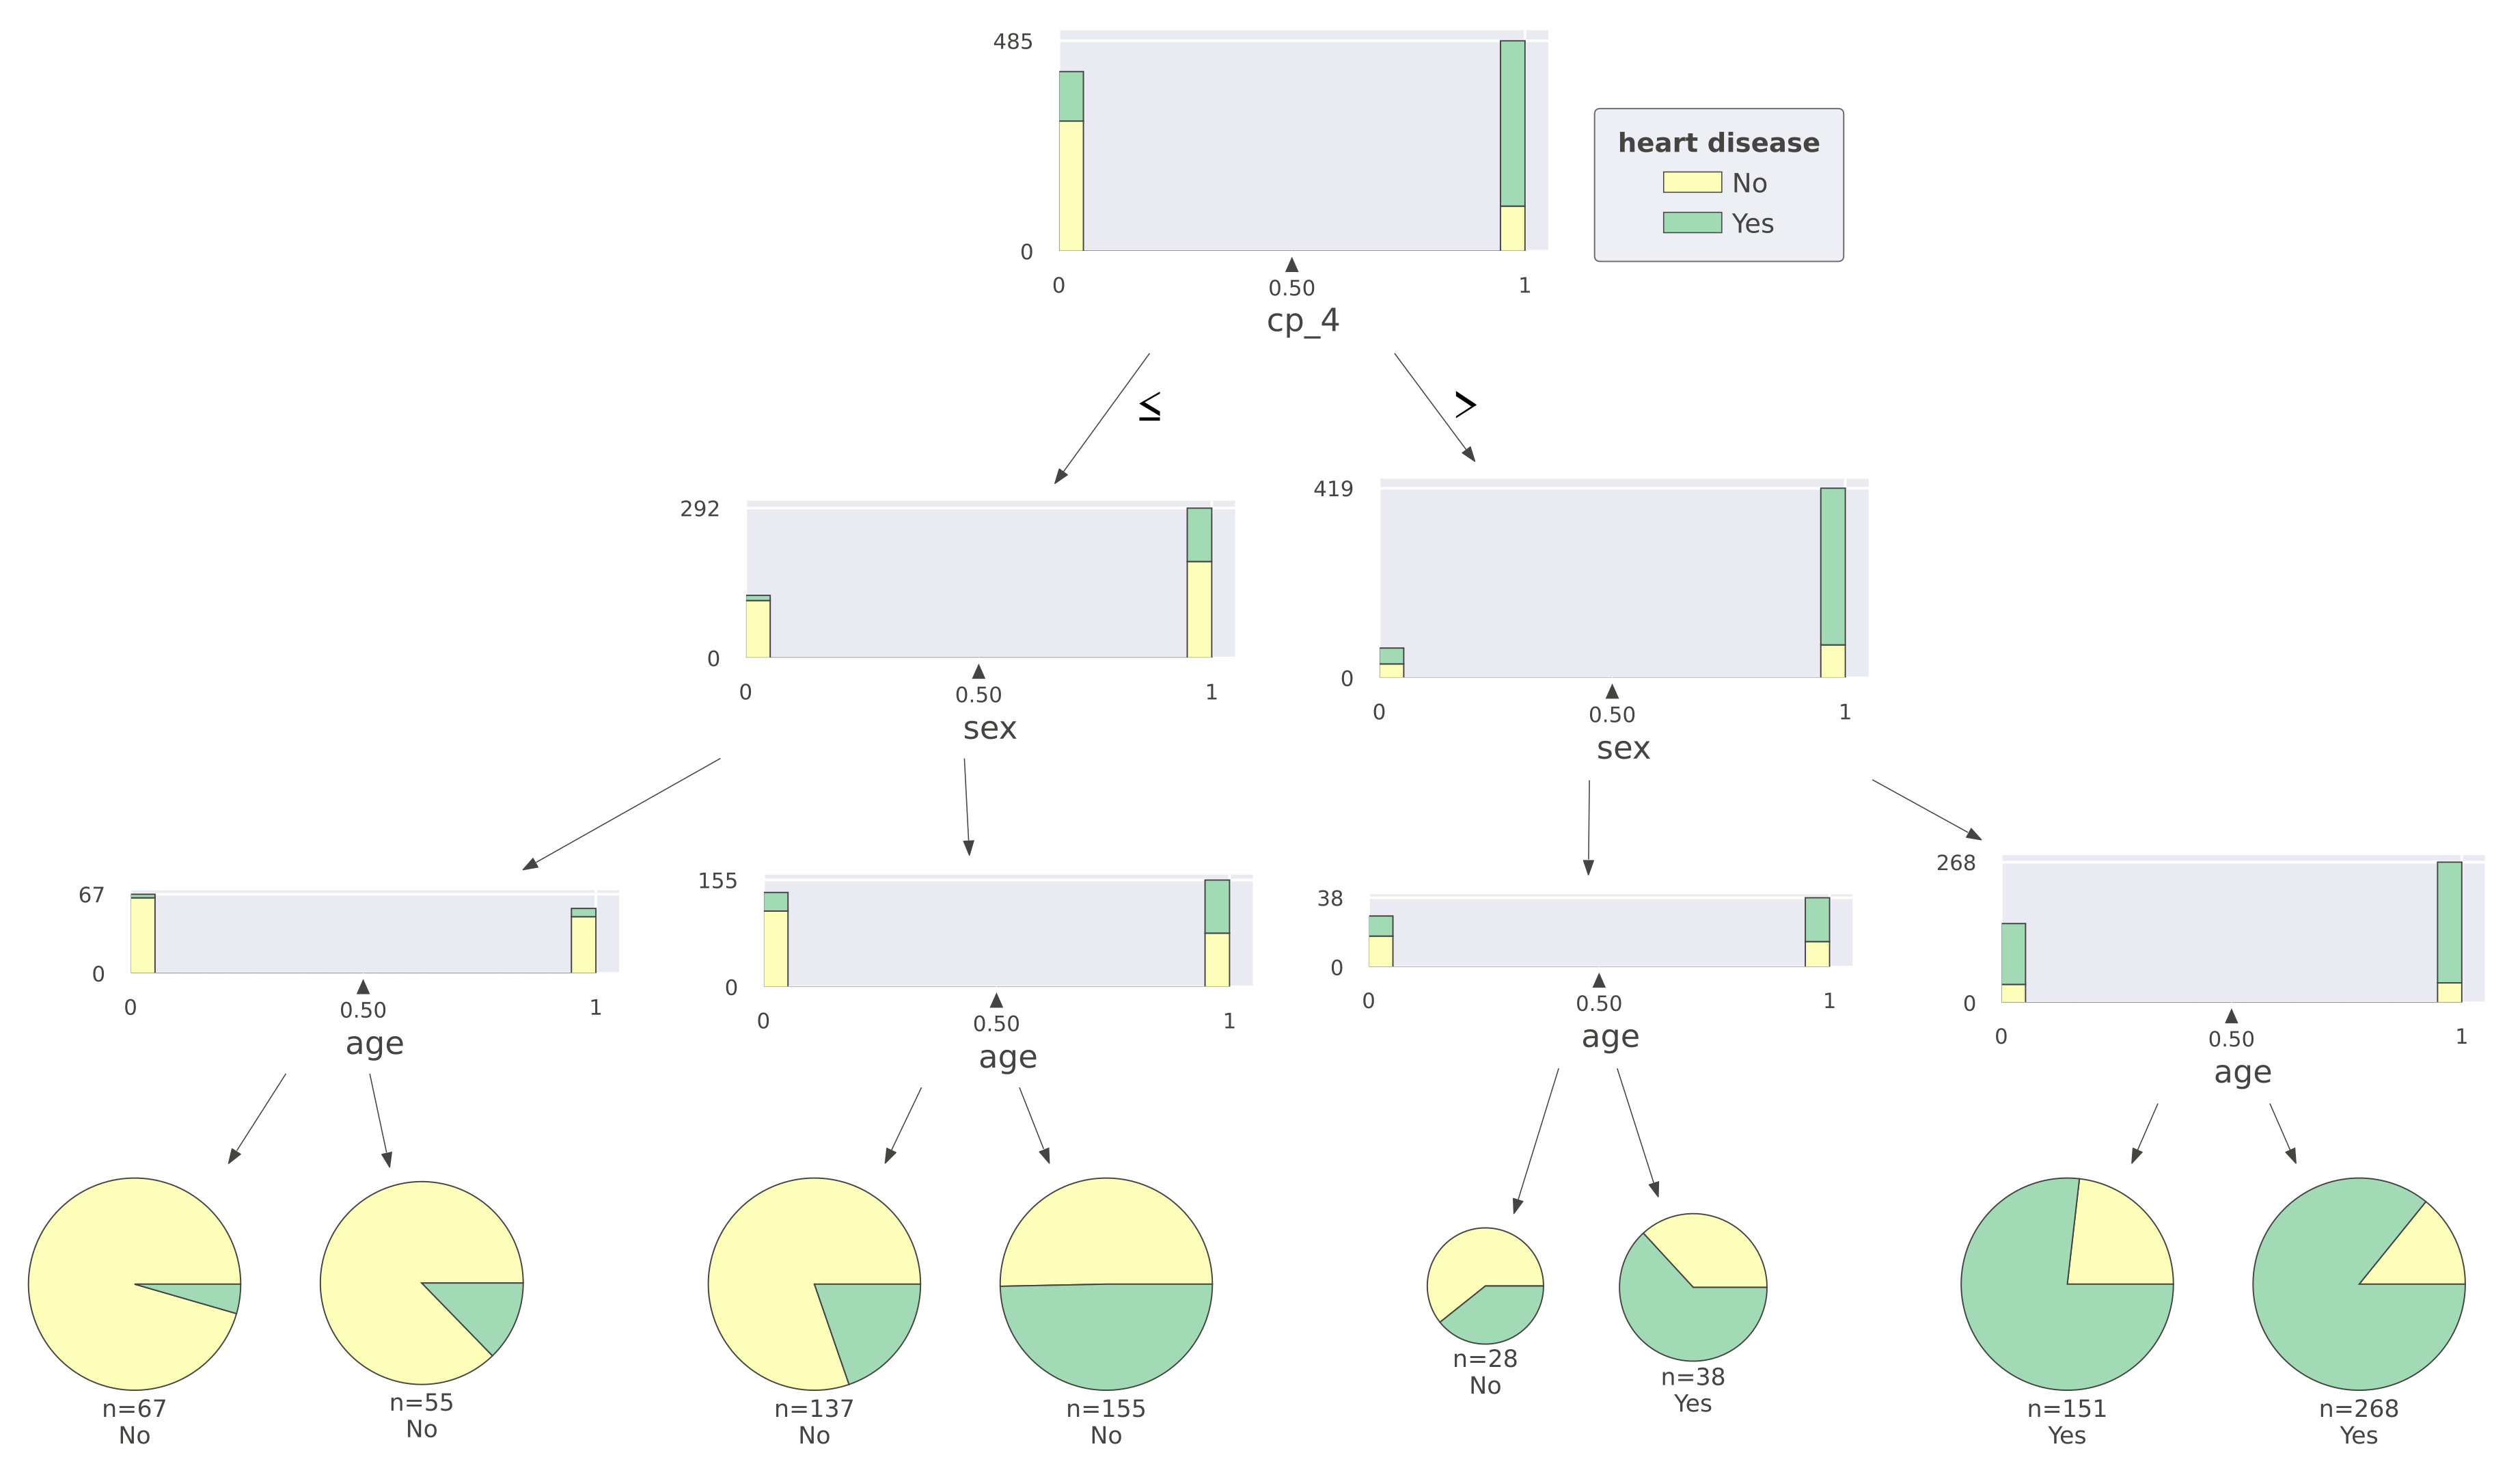
\includegraphics[width=\textwidth]{images/DecisionTree.png}
	\caption{Decision tree visualized}
	\label{fig:DecisionTree}
\end{figure}


\todo{ich glaubve hier fehlen einige Kommas, evtl lassen wir den ganzen report nochmal durch einen Grammar checker laufen}